\documentclass[a4paper,12pt]{article}

\usepackage[top=3cm, bottom=2cm, left=3cm, right=2cm]{geometry}
\usepackage[utf8]{inputenc}
\usepackage[portuguese]{babel}
\usepackage{booktabs}
\usepackage{multirow}
\usepackage{graphicx}
\usepackage{longtable}
\usepackage{verbatim}

\usepackage{float}
\floatstyle{ruled}
\newfloat{program}{thp}{lop}
\floatname{program}{Script}

\title{Serviços de Rede e de Sistema \\
Endereçamento IP e serviço DNS}

\author{André Fernandes (ei03107) \and Pedro Batista (ext10392)}

\begin{document}

\maketitle

\section{Endereçamento}
\subsection{Projectar o esquema de endereçamento da rede da empresa,
usando do bloco de endereços acima, apenas os blocos de endereços com
o tamanho necessário para cada rede. Justifique.}

\begin{table}[h]
   \centering

   \begin{tabular}{ l | c | c | c }
      \toprule
      \textbf{Descrição} & \textbf{Quantidade} & \textbf{Total} & \textbf{Intervalo de Endereços} \\\hline

      \multicolumn{4}{c}{\textit{Rede Edifício Sede (VLAN100)}} \\ \hline
      Estações & 300 & 300 & 192.168.0.0 - 192.168.1.255 \\ \hline

      \multicolumn{4}{c}{\textit{Loja 1 (VLAN21X)}} \\\hline
      VLAN210 & 25 & 25 & 192.168.2.0 - 192.168.2.31 \\\hline
      VLAN211 & 17 & 17 & 192.168.2.32 - 192.168.2.63 \\\hline

      \multicolumn{4}{c}{\textit{Loja 2 (VLAN22X)}} \\\hline
      VLAN220 & 25 & 25 & 192.168.2.64 - 192.168.2.95 \\\hline
      VLAN221 & 17 & 17 & 192.168.2.96 - 192.168.2.127\\\hline

      \multicolumn{4}{c}{\textit{Loja 3 (VLAN23X)}} \\\hline
      VLAN230 & 25 & 25 & 192.168.2.128 - 192.168.2.159 \\\hline
      VLAN231 & 17 & 17 & 192.168.2.160 - 192.168.2.191 \\\hline

      \multicolumn{4}{c}{\textit{Armazém (VLAN300)}} \\\hline
      Estações & 17 & \multirow{2}{*}{18} & \multirow{2}{*}{192.168.2.192 - 192.168.2.223} \\\cline{1-2}
      Servidor & 1 & \\\hline 

      \multicolumn{4}{c}{\textit{DMZ (VLAN400)}} \\\hline
      Servidores & 3 & 3 & 20.49.51.160 - 20.49.51.168 \\\hline

      \multicolumn{4}{c}{\textit{Rede de Servidores (VLAN500)}} \\\hline
      Servidores & 3 & 3 & 192.168.2.224 - 192.168.2.231 \\\hline
      \bottomrule

   \end{tabular}
   \caption{Esquema de endereçamento.}
   \label{tab:enderecamento_esquema}
\end{table}

\subsection{Apresente os vários endereços (identificação da rede e broadcast) e as respectivas máscaras para cada uma das redes.}
\subsection{Atribua endereços aos servidores indicados e às gateways de cada rede local.
As boas práticas recomendam que os servidores tenham os endereços mais
baixos da rede, por exemplo o mais baixo será o servidor de DNS, e a gateway
o mais alto (antes do broadcast).}

\begin{center}
\begin{longtable}{ l | c }
   \caption{Endereços dos servidores.} \label{grid_mlmmh} \\
   \toprule
   \endfirsthead

   \endhead

   \multicolumn{2}{l}{ Continua na próxima página. } \\
   \endfoot

   \bottomrule
   \endlastfoot

   \multicolumn{2}{c}{Rede Edifício Sede} \\\hline 
   Mascara & 255.255.254.0 \\\hline
   Rede & 192.168.0.0 \\\hline 
   Gateway & 192.168.1.254 \\\hline
   Broadcast & 192.168.1.255 \\\hline 

   \multicolumn{2}{c}{Loja 1} \\\hline 
   Mascara & 255.255.255.224 \\\hline

   SubRede1 & 192.168.2.0 \\\hline 
   Broadcast SubRede1 & 192.168.2.31 \\\hline
   Gateway SubRede1 & 192.168.2.30 \\\hline

   SubRede2 & 192.168.2.32 \\\hline 
   Broadcast SubRede2 & 192.168.2.63 \\\hline
   Gateway SubRede2 & 192.168.2.62 \\\hline

   Servidor SubRede1 (DNS e Proxy) & 192.168.2.1 \\\hline
   Servidor SubRede2 (DNS e Proxy) & 192.168.2.33 \\\hline

   \multicolumn{2}{c}{Loja 2} \\\hline 
   Mascara & 255.255.255.224 \\\hline

   SubRede1 & 192.168.2.68 \\\hline 
   Broadcast SubRede1 & 192.168.2.95 \\\hline
   Gateway SubRede1 & 192.168.2.94 \\\hline

   SubRede2 & 192.168.2.96\\\hline 
   Broadcast SubRede2 & 192.168.2.127 \\\hline
   Gateway SubRede2 & 192.168.2.126\\\hline

   Servidor SubRede1 (DNS e Proxy) & 192.168.2.69 \\\hline
   Servidor SubRede2 (DNS e Proxy) & 192.168.2.97 \\\hline

   \multicolumn{2}{c}{Loja 3} \\\hline 
   Mascara & 255.255.255.224 \\\hline

   SubRede1 & 192.168.2.128 \\\hline 
   Broadcast SubRede1 & 192.168.2.159 \\\hline
   Gateway SubRede1 & 192.168.2.154\\\hline

   SubRede2 & 192.168.2.160\\\hline 
   Broadcast SubRede2 & 192.168.2.191 \\\hline
   Gateway SubRede2 & 192.168.2.190 \\\hline

   Servidor SubRede1 (DNS e Proxy) & 192.168.2.129 \\\hline
   Servidor SubRede2 (DNS e Proxy) & 192.168.2.161 \\\hline

   \multicolumn{2}{c}{Armazém} \\\hline 
   Mascara & 255.255.255.224 \\\hline
   Rede & 192.168.2.192 \\\hline 
   Broadcast & 192.168.2.223 \\\hline 
   Gateway & 192.168.2.222 \\\hline
   Servidor (Cache DNS) & 192.168.2.193 \\\hline
   %      Loja 1 &             192.168.2.0   & 192.168.2.63  &      \multirow{3}{*}{255.255.255.192} \\\cline{1-3}
   %      Loja 2 &             192.168.2.64  & 192.168.2.127 &      \\\cline{1-3}
   %      Loja 3 &             192.168.2.128 & 192.168.2.191 &      \\\hline
   %      Armazém &            192.168.2.192   & 192.168.2.223 &      255.255.254.224 \\

   \multicolumn{2}{c}{Rede de Servidores Internos} \\\hline 
   Mascara & 255.255.255.248 \\\hline
   Rede & 192.168.2.224 \\\hline 
   Broadcast & 192.168.2.231 \\\hline 
   Gateway & 192.168.2.230 \\\hline
   Servidor DNS & 192.168.2.225 \\\hline
   Servidor WWW & 192.168.2.226 \\\hline
   Servidor MAIL & 192.168.2.227 \\\hline

   \multicolumn{2}{c}{DMZ} \\\hline 
   Mascara & 255.255.255.248 \\\hline
   Rede & 29.49.51.160 \\\hline 
   Broadcast & 20.49.51.167 \\\hline 
   Gateway & 20.49.51.166 \\\hline
   Servidor DNS & 20.49.51.161 \\\hline
   Servidor WWW & 20.49.51.162 \\\hline
   Servidor MAIL & 20.49.51.163 \\\hline
\end{longtable}
\end{center}

\subsection{Assumindo a atribuição de endereços que fez anteriormente, configure na sua
bancada uma topologia de rede que represente a rede de servidores do edifício
sede, as redes de uma loja e a do armazém.}

A Figura~\ref{fig:topologia} mostra a organização dos recursos disponibilizados
para a implementação da rede proposta. O Script~\ref{verb:gnus} mostra a configuração
aplicada em cada computador da bancada. No switch e no router as configurações
aplicadas são mostradas nos Scripts \ref{verb:swicth_vlan}, \ref{verb:switch_ports}, e \ref{verb:router}.

\begin{figure}[htp]
   \begin{center}
      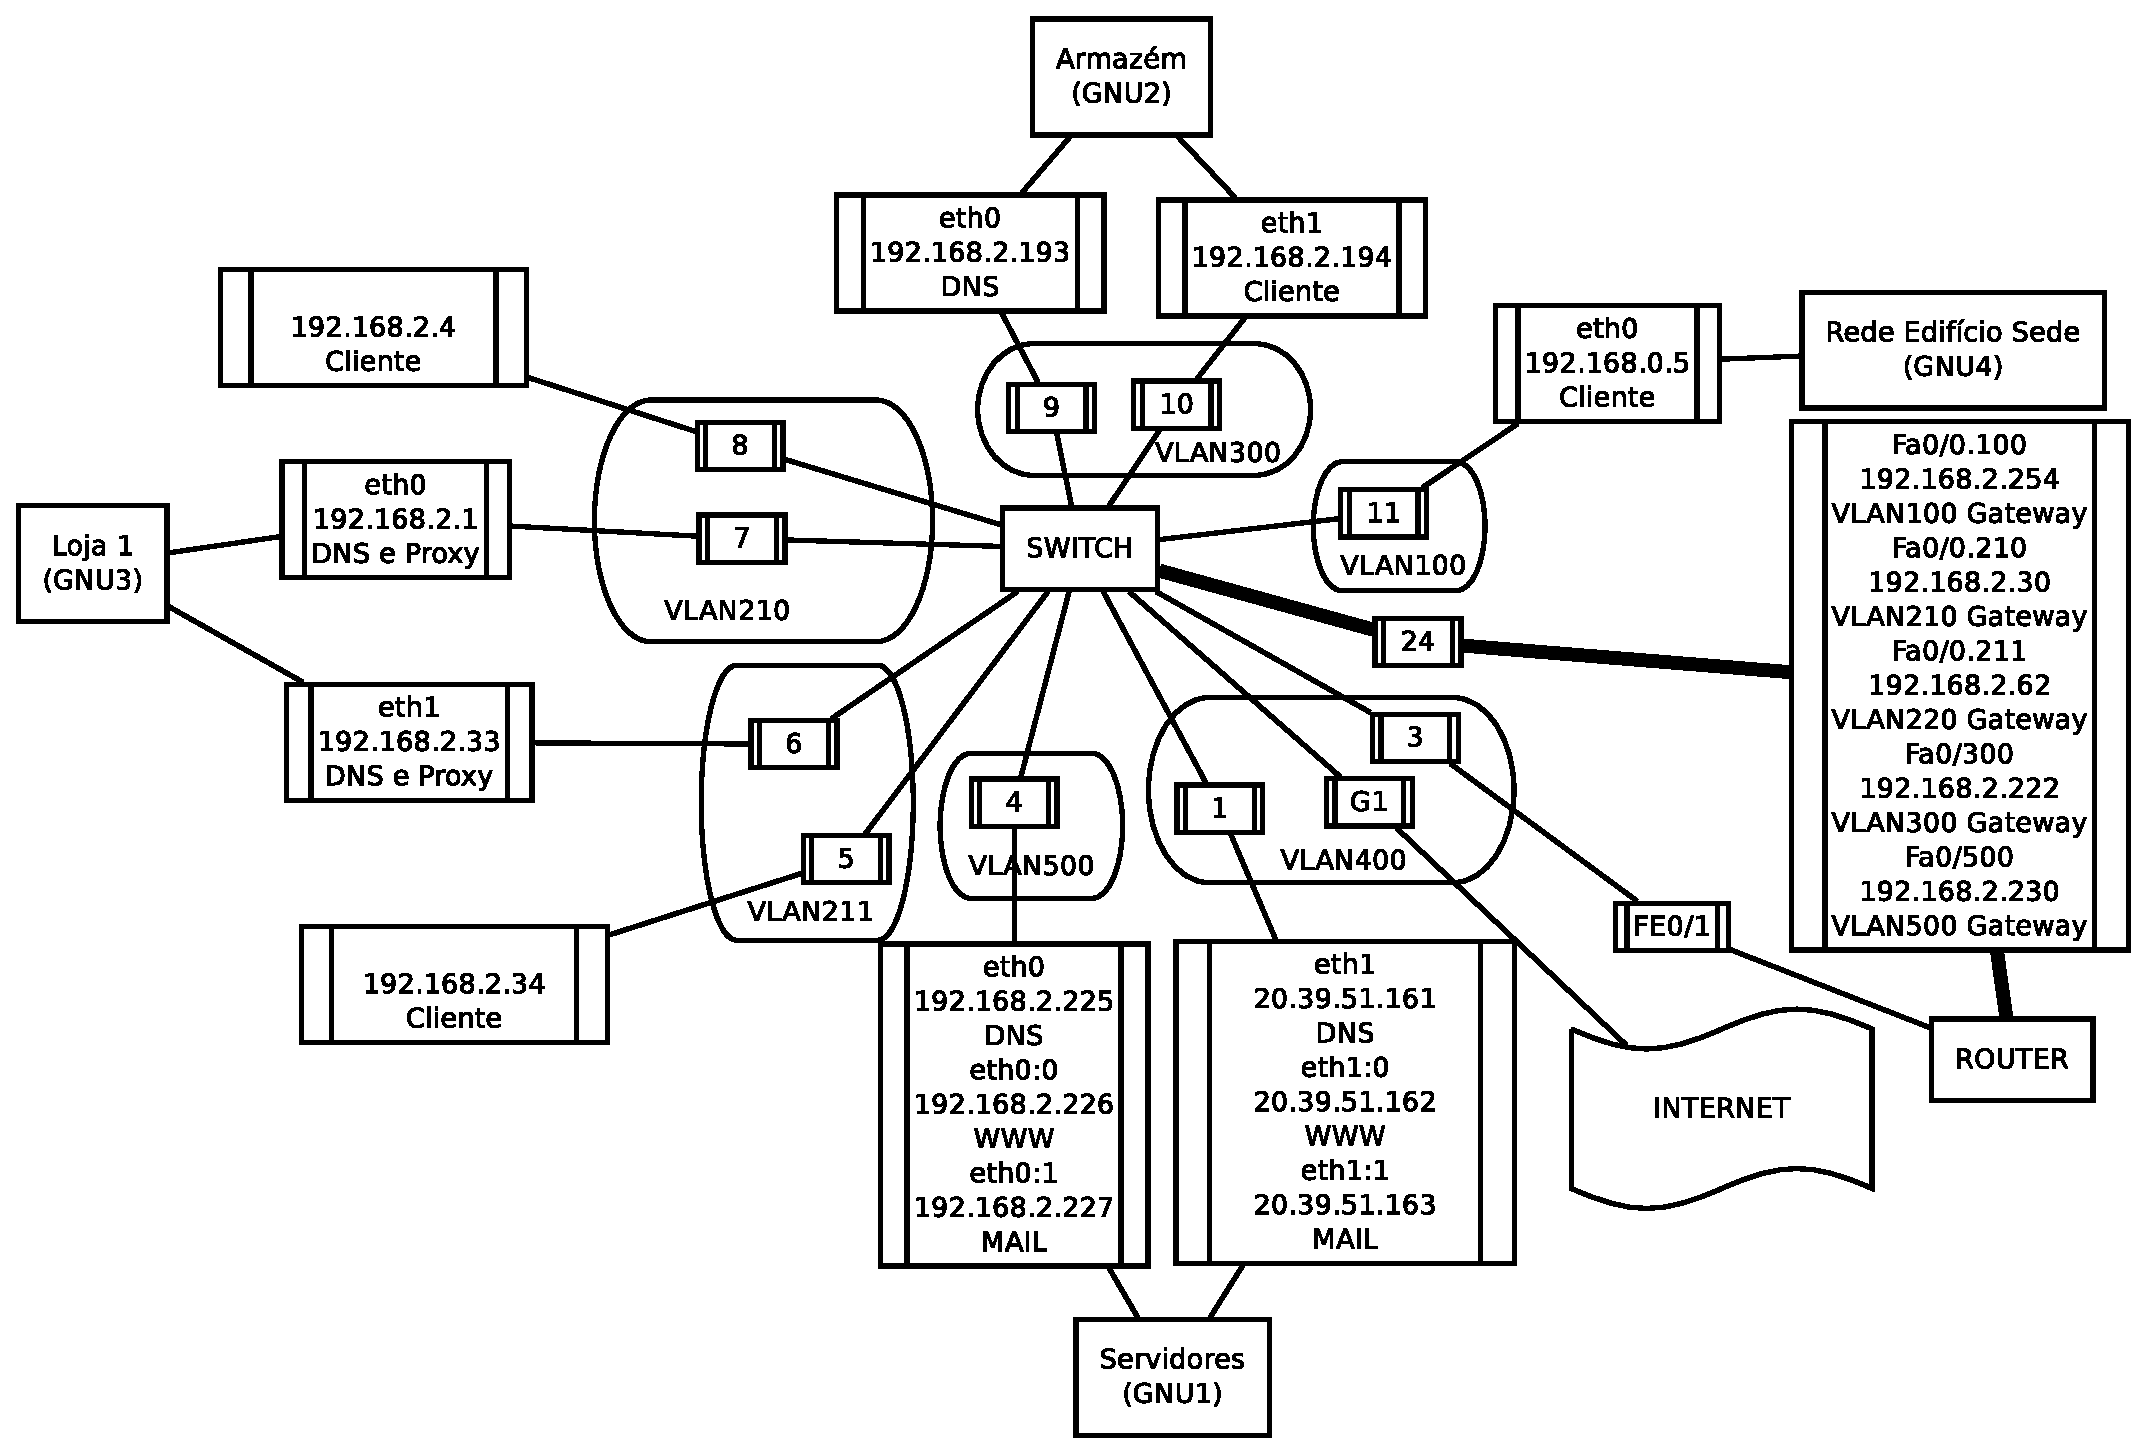
\includegraphics[height=300pt]{topologia}
   \end{center}
   \caption{Topologia da rede.}
   \label{fig:topologia}
\end{figure}

\begin{program}
   \verbatiminput{configure_gnus.txt}
   \caption{Configuração dos computadores.}
   \label{verb:gnus}
\end{program}

\begin{program}
   \verbatiminput{configure_switch_vlan.txt}
   \caption{Criação das VLANs no switch.}
   \label{verb:swicth_vlan}
\end{program}

\begin{program}
   \verbatiminput{configure_switch_ports.txt}
   \caption{Atribuição de portas as VLANs no switch.}
   \label{verb:switch_ports}
\end{program}

\begin{program}
   \verbatiminput{configure_router.txt}
   \caption{Configuração do router.}
   \label{verb:router}
\end{program}

\section{DNS}
\subsection{Configure uma solução de “split DNS” com um servidor primário para o
domínio qquma.pt na Intranet e o outro será o que estará disponível para a
Internet com a informação dos serviços/servidores da DMZ (configure o
servidor de DNS da Intranet para fazer forward para o servidor de DNS
externo com conectividade à Internet, ou alternativamente configure um
servidor com “vistas”).}

Os Scripts \ref{verb:s_co},~\ref{verb:s_op},~\ref{verb:s_dbin} e~\ref{verb:s_dbout}
mostram as configurações do BIND, com 2 Views, uma para a rede externa e outra para a rede interna para o domínio qquma.pt. E a configuração do servidor central como slave para o domínio loja1.qquma.pt.

\begin{program}
   \verbatiminput{bind_s/named.conf}
   \caption{Configuração DNS do servidor central.}
   \label{verb:s_co}
\end{program}

\begin{program}
   \verbatiminput{bind_s/named.conf.options}
   \caption{Configuração do servidor central DNS do domínio qquma.pt como servidor DNS de cache para o domínio loja1.qquma.pt.}
   \label{verb:s_op}
\end{program}

\begin{program}
   \verbatiminput{bind_s/db.internal.qquma.pt}
   \caption{Tabela de endereços internos para o servidor central.}
   \label{verb:s_dbin}
\end{program}

\begin{program}
   \verbatiminput{bind_s/db.external.qquma.pt}
   \caption{Tabela de endereços externos para o servidor central.}
   \label{verb:s_dbout}
\end{program}

\subsection{Configure para o sub-domínio das redes da loja o respectivo servidor DNS e
coloque o servidor DNS do domínio da empresa como servidor secundário
(slave) deste.}

Nos Scripts~\ref{verb:l_co},~\ref{verb:l_op} e~\ref{verb:l_db} são
mostradas as configurações aplicadas para o servidor DNS da loja1.

\begin{program}
   \verbatiminput{bind_l/named.conf.local}
   \caption{Configurações do servidor DNS da loja1.}
   \label{verb:l_co}
\end{program}

\begin{program}
   \verbatiminput{bind_l/named.conf.options}
   \caption{Configuração do servidor DNS da loja1 para trabalhar como servidor cache do domínio qquma.pt e nomes externos.}
   \label{verb:l_op}
\end{program}

\begin{program}
   \verbatiminput{bind_l/db.loja1.qquma.pt}
   \caption{Tabela de endereços para o servidor DNS da loja1.}
   \label{verb:l_db}
\end{program}

\subsection{Na rede do armazém configure o servidor de cache de DNS previsto.}
O servidor de cache de DNS no armazém foi configurado segundo o Script~\ref{verb:a_op}.

\begin{program}
   \verbatiminput{bind_a/named.conf.options}
   \caption{Configuração do servidor do Armazém.}
   \label{verb:a_op}
\end{program}

\subsection{Active a geração de logs do BIND no(s) servidor(es) e teste as configurações.
Apresente o extracto do log demonstrativo do bom funcionamento das
configurações.}

Abaixo são apresentadas uma série de respostas, por parte dos 3 servidores de DNS, às requisições das demais máquinas da rede.

\begin{program}
   \verbatiminput{logs/a_s.dig}
   \caption{Requisição do armazém para o servidor central.}
   \label{verb:a_s}
\end{program}

\begin{program}
   \verbatiminput{logs/e_s.dig}
   \caption{Requisição da rede do edifício sede para o servidor central.}
   \label{verb:e_s}
\end{program}

\begin{program}
   \verbatiminput{logs/l_s.dig}
   \caption{Requisição da rede da loja1 para o servidor central.}
   \label{verb:l_s}
\end{program}

\begin{program}
   \verbatiminput{logs/s_s.dig}
   \caption{Requisição do servidor central para ele mesmo.}
   \label{verb:s_s}
\end{program}

\begin{program}
   \verbatiminput{logs/a_l.dig}
   \caption{Requisição do armazém para o servidor da loja1.}
   \label{verb:a_l}
\end{program}

\begin{program}
   \verbatiminput{logs/e_l.dig}
   \caption{Requisição da rede do edifício sede para o servidor da loja1.}
   \label{verb:e_l}
\end{program}

\begin{program}
   \verbatiminput{logs/l_l.dig}
   \caption{Requisição do servidor da loja1 para ele mesmo.}
   \label{verb:l_l}
\end{program}

\begin{program}
   \verbatiminput{logs/s_l.dig}
   \caption{Requisição do servidor central para o servidor da loja1.}
   \label{verb:s_l}
\end{program}

\begin{program}
   \verbatiminput{logs/a_a.dig}
   \caption{Requisição do servidor do armazém para ele mesmo.}
   \label{verb:a_a}
\end{program}

\begin{program}
   \verbatiminput{logs/e_a.dig}
   \caption{Requisição da rede do edifício sede para o servidor do armazém.}
   \label{verb:e_a}
\end{program}

\begin{program}
   \verbatiminput{logs/l_a.dig}
   \caption{Requisição da rede da loja1 para o servidor do armazém.}
   \label{verb:l_a}
\end{program}

\begin{program}
   \verbatiminput{logs/s_a.dig}
   \caption{Requisição do servidor central para o servidor do armazém.}
   \label{verb:s_a}
\end{program}
\end{document}
